% !TeX root = ..

% Часть I Глава 1

\chapter{
  МОДЕЛИРОВАНИЕ МАРШРУТА ИНСТРУМЕНТА
  ДЛЯ~МАШИН ФИГУРНОЙ ЛИСТОВОЙ РЕЗКИ
  С~ЧИСЛОВЫМ ПРОГРАММНЫМ УПРАВЛЕНИЕМ.
  ОСНОВНЫЕ~ПОНЯТИЯ И~ЗАДАЧИ
}
%\setcounter{section}{1}\setcounter{subsection}{1}
\setcounter{chapter}{1}
\setcounter{equation}{0}

% !TeX root = ../mat_mod2.tex

\section{\protect\raggedright
  Технологии и техники листовой резки на машинах с ЧПУ
}
\label{sect:1.1}
\setcounter{equation}{0}

В машиностроении,
производстве металлоконструкций
и других отраслях промышленности существенная часть продукции
изготавливается из заготовок,
получаемых из листовых материалов на различном технологическом оборудовании.
К такому оборудованию относятся, в частности,
используемые на предприятиях отечественные и зарубежные
системы автоматизированного проектирования (САПР),
предназначенные для разработки управляющих программ (УП)
для машин листовой резки с ЧПУ
(т. н. \textit{Computer-Aided Manufacturing},
\textit{CAM}-системы),
которые
обеспечивают автоматизацию процесса разработки УП,
однако не позволяют решить многие оптимизационные задачи.
При этом при моделировании маршрута инструмента пользователям
САПР часто приходится применять интерактивные методы проектирования УП,
поскольку алгоритмы генерации УП,
реализованные в автоматическом режиме проектирования,
во многих случаях не позволяют генерировать оптимальные управляющие программы,
а также обеспечить соблюдение некоторых технологических требований листовой резки.
В качестве критериев оптимизации имеются в виду время резки и
некоторые другие стоимостные характеристики процесса листовой резки.
Проблема разработки методов, алгоритмов и соответствующего программного обеспечения,
позволяющих в автоматическом режиме оптимизировать параметры
процесса резки заготовок из листовых материалов на машинах с ЧПУ,
включая алгоритмы маршрутизации движения инструмента,
которые бы обеспечивали минимизацию времени резки и стоимости процесса,
остается актуальнейшей задачей раскройно-заготовительного производства.

Рассмотрим понятие маршрута инструмента (маршрута резки)
применительно к некоторым технологиям фигурной листовой резки.
В настоящее время в промышленном производстве
единичного и мелкосерийного типа для раскроя листовых материалов
используются в основном следующие технологии:
лазерная, плазменная, газовая и гидроабразивная.
Целесообразность их применения определяется различными технологическими факторами,
например, свойствами раскраиваемого материала,
экономическими требованиями к процессу резки,
требованиями к качеству реза и пр.
Эти и некоторые другие технологии резки предполагают,
что для сохранения требуемой геометрии заготовки
траектория движения режущего инструмента не совпадает
с граничным контуром заготовки,
а задается некоторой эквидистантой этого контура,
поскольку часть материала вырезается (<<сгорает>>, <<вымывается>> и пр.)
в процессе резки.
Как правило, дистанция между эквидистантным контуром,
по которому осуществляется резка, и граничным контуром заготовки определяется величиной,
равной половине ширины реза.
Эта величина зависит от выбранной технологии резки,
толщины и марки материала, заданной скорости резки
и особенностей конкретного технологического оборудования,
используемого для резки.

Еще одна особенность листовой резки –
необходимость предварительной врезки (пробивки)
материала перед процессом резки непосредственно
по эквидистантному контуру заготовки.
Пробивка материала сопровождается дополнительными
деформациями материала в точке врезки,
поэтому производится на расстоянии (дистанции)
от контура заготовки большем,
чем дистанция до эквидистантного контура за исключением случаев,
когда для точек врезки в листовом материале механическим способом
готовятся (например, просверливаются)
отверстия.
Врезка может также осуществляться
непосредственно на границе материала
(<<врезка с края листа>>).
В этом случае достигается уменьшение
деформаций материала и сокращается время врезки.

На рис. \ref{standard-cutting}.
показан
один из способов резки заготовки
(стандартная техника).

\begin{figure}[h]
  \begin{center}
  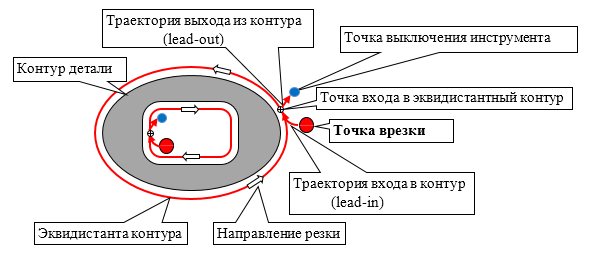
\includegraphics[width=0.9\textwidth]{cutting-path.png}
  \caption{Схема стандартной техники резки (резка по замкнутому контуру)}
  \label{standard-cutting}
  \end{center}
\end{figure}

Если используется стандартная техника резки,
то в этом случае каждый замкнутый контур вырезается целиком,
и после резки одного контура переход к следующей точке врезки
происходит с выключенным инструментом на холостом ходу.
При этом точка выключения инструмента
в общем случае
может не совпадать с точкой входа в эквидистантный контур заготовки,
по которому осуществляется резка, и также,
как и точка врезки,
может лежать вне заданного эквидистантного контура.
Во многих случаях допускается программирование точки выключения
инструмента непосредственно на эквидистантном контуре.

Стратегия минимизации тепловых деформаций при термической резке
и требования к качеству реза порождают необходимость управления
не только выбором точек врезки,
но и управлением траекторией подхода к контуру
(\textit{lead-in})
и способом выхода из контура
(\textit{lead-out}).
В зависимости от конкретных условий
(вида термической резки, марки и толщины материала,
скорости резки, геометрической формы контура и пр.)
подход к контуру может осуществляться по дуге окружности,
касательная к которой совпадает с касательной к контуру в точке входа,
либо производиться по прямой линии
(например, по наикратчайшему расстоянию до контура).
Соответственно и после завершения резки выход из контура
также может осуществляться с включенным инструментом
(либо по дуге, либо по прямой линии).
Необходимость выхода из контура с включенным
инструментом может быть вызвана тем,
что в точке выключения инструмента может возникнуть
<<вырыв>> или оплавление части материала,
что приводит к искажению геометрии заготовки.
Уменьшение эффекта деформации заготовок обеспечивает
также врезка в <<угловые>> точки заготовок
(рис.~\ref{corner}).

\begin{figure}[h]
  \begin{center}
  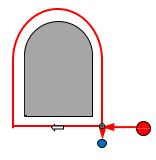
\includegraphics[width=0.3\textwidth]{corner.png}
  \caption{Пример врезки <<в угол>>}
  \label{corner}
  \end{center}
\end{figure}

Примером нестандартной техники
может служить <<цепная>> резка,
которая заключается в резке нескольких контуров с
использованием одной точки врезки.
При этом каждый контур,
как и в случае применения стандартной техники резки,
вырезается целиком.
На рис.~\ref{chain}
показан пример схемы резки двух заготовок,
в которой резка внешних контуров обеих заготовок
производится без выключения инструмента
с использованием только одной точки врезки.

Перемещение инструмента в точку врезки
в этом примере начинается из начальной точки на холостом ходу,
а после завершения резки последнего контура
предусмотрен возврат инструмента в начальную точку.

\begin{figure}[h]
  \begin{center}
  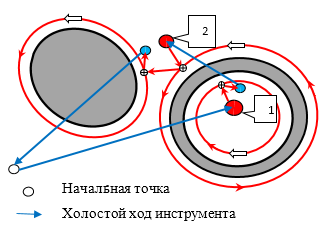
\includegraphics[width=0.5\textwidth]{chain.png}
  \caption{
    Пример схемы резки двух заготовок
    с~использованием стандартной
    и~<<цепной>> техники резки}
  \label{chain}
  \end{center}
\end{figure}

На практике применяется также техника резки
замкнутого контура заготовок по частям
с использованием нескольких точек врезки
с целью формирования т. н. <<перемычек>>
(рис.~\ref{jumper}),
а также используются другие специальные приемы,
целью которых является оптимизация различных параметров,
характеризующих процесс резки,
и соблюдение необходимых технологических требований резки.
Техника резки <<перемычка>> предусматривает
оставление невырезанной части контура заготовки,
обычно небольшого прямолинейного отрезка или нескольких отрезков
с резкой этих отрезков после завершения резки оставшейся части контура.
Этот прием применяется с целью уменьшения деформаций материала
при термической резке заготовок, склонных к термическим деформациям,
в частности, длинномерных заготовок.

\begin{figure}[h]
  \begin{center}
  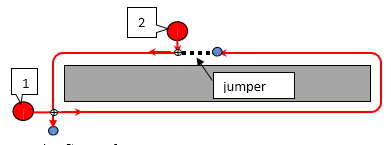
\includegraphics[width=0.5\textwidth]{jumper.png}
  \caption{Схема формирования перемычки на контуре при резке полосы}
  \label{jumper}
  \end{center}
\end{figure}

На рис.~\ref{saber} показан пример искажения геометрической формы
(получения т. н. формы <<сабли>>)
и~изменения размера длинномерной прямоугольной заготовки,
вырезаемой без использования техники <<перемычка>>.

\begin{figure}[h]
  \begin{center}
  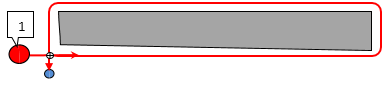
\includegraphics[width=0.5\textwidth]{saber.png}
  \caption{
    Результат изменнения формы
    и~размера прямоугольной заготовки
    при~термической резке
    }
  \label{saber}
  \end{center}
\end{figure}

На рис.~\ref{bridge}
приведен пример использования техники <<мост>>,
предполагающей  частичную резку замкнутого контура
заготовки с последующим завершением резки контура
после резки контура другой заготовки или
группы контуров других заготовок.
Эта техника используется при резке двух или
нескольких рядом расположенных заготовок и
предусматривает переход по короткой траектории (<<мосту>>)
к резке другой заготовки и возврат к первому контуру
по этой же траектории для завершения процесса резки.
Так же, как и <<перемычки>>,
мосты существенно уменьшают тепловые деформации материала,
особенно при резке длинномерных заготовок,
кроме того, сокращают число точек врезки.

\begin{figure}[h]
  \begin{center}
  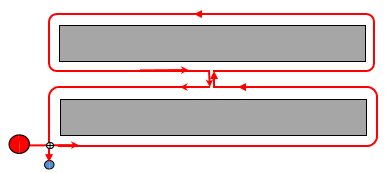
\includegraphics[width=0.5\textwidth]{bridge.png}
  \caption{Схема резки двух полос с использованием техники <<мост>>}
  \label{bridge}
  \end{center}
\end{figure}

Разновидностью техники <<мост>> можно считать технику <<змейка>>,
показанную на рис.~\ref{snake},
в которой также используется прием
частичной резки контура и резки
нескольких заготовок без выключения инструмента.

\begin{figure}[h]
  \begin{center}
  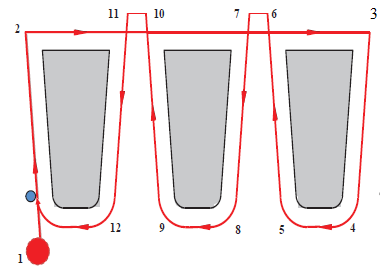
\includegraphics[width=0.7\textwidth]{snake.png}
  \caption{Схема резки <<змейка>>}
  \label{snake}
  \end{center}
\end{figure}

Для уменьшения длины рабочего хода инструмента
применяют т. н. <<совмещенный>> рез.
Он используется для вырезки заготовок,
которые содержат прямолинейные отрезки в контуре
и которые в процессе раскроя размещаются таким образом,
что имеют общую границу по одному из таких прямолинейных отрезков.
Общая прямолинейная граница позволяет размещать
заготовки с половинным припуском на рез
(т. е. на ширину реза),
поскольку режется только один раз,
что экономит материал и сокращает суммарную
длину резки на величину совмещенного реза.
Совмещенный рез реализован, в частности,
в технике резки <<восьмерка>>,
применяемой для резки двух одинаковых заготовок
(рис.~\ref{8}).
В этой технике используется также идея цепной резки.

\begin{figure}[h]
  \begin{center}
  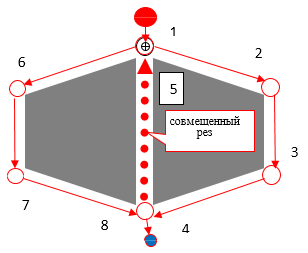
\includegraphics[width=0.6\textwidth]{8.png}
  \caption{Схема резки <<восьмеркой>> двух заготовок}
  \label{8}
  \end{center}
\end{figure}

Основные технологические требования
фигурной резки на машинах с ЧПУ обусловлены
необходимостью учета возникающих деформаций
материала и искажения геометрических размеров
вырезаемых заготовок при использовании
термических технологий резки.
Применение специальных техник позволяет
уменьшить эффект искажения геометрии,
который особенно значителен при
использовании газовой и плазменной технологий.

При использовании любой техники резки маршрут инструмента
машины с ЧПУ для фигурной листовой резки
включает в себя следующие компоненты:
\begin{itemize}
  \item точки врезки;
  \item рабочий ход инструмента;
  \item точки выключения инструмента;
  \item линейное перемещение инструмента на холостом ходу
  между точкой выключения инструмента и следующей точкой врезки.
\end{itemize}

При разработке управляющей программы
первое перемещение инструмента обычно
программируется, как на рис.~\ref{chain},
из начальной точки.

Отметим, что некоторые машины фигурной листовой
резки с ЧПУ могут быть укомплектованы
специальным видом инструмента,
т. н. трехрезаковым блоком для вырезания
из листа заготовок с одновременной разделкой
кромок поверхности реза для последующей сварки.
Врезка в материал для такого инструмента
программируется специальными способами.

Введем некоторые определения,
касающиеся понятия маршрута резки.
В дальнейшем при формальном обозначении
математических и геометрических категорий
мы будем использовать стандартную
теоретико-множественную символику.
Ее детальное описание дано в разделе 3.1.
%%% TODO! Fix reference ^^^^^^^^^^^^^^
Введем следующее определение.

\begin{opred}
\label{def:cutting-segment}
{\bf Сегментом резки}
$S=MM^*$
будем называть траекторию рабочего хода
инструмента между точкой врезки
$M$
и соответствующей ей точкой выключения инструмента
$M^*$.
Геометрически сегмент резки представляет собой
определенную на эвклидовой плоскости
$\mathbb R \times \mathbb R$
кривую.
$(S \subset \mathbb R \times \mathbb R;
M=(x,y) \in \mathbb R \times \mathbb R,
M^* =(x^*,y^*)\in \mathbb R \times \mathbb R)$.
Будем также полагать,
что в каждой точке траектории определено направление движения инструмента.
Заметим, что если сегмент резки не содержит замкнутых контуров,
то направление движения резки в каждой точке траектории
однозначно определяется начальной точкой сегмента
(точкой врезки).
Замкнутые контуры в траектории рабочего хода инструмента
могут появляться не только в результате резки контуров заготовок,
но и при программировании т. н. петель,
которые используются для повышения качества реза.
\end{opred}

Используя понятие сегмента резки,
все техники фигурной резки на машинах с ЧПУ
можно разделить на три класса.
\begin{enumerate}
  \item
  {\it Резка по замкнутому контуру (стандартная техника)}:
  в этом случае сегмент резки содержит
  ровно один замкнутый эквидистантный контур заготовки,
  который вырезается целиком.
  \item
  {\it Мультисегментная резка контура}:
  в этом случае для вырезки одного контура
  используются не менее двух сегментов резки.
  \item
  {\it Мультиконтурная резка}:
  резка предполагает вырезку нескольких
  контуров в одном сегменте.
\end{enumerate}

Примерами мультиконтурной резки являются,
в частности, приведенные выше техники резки:
<<цепная резка>>, <<мост>>, <<змейка>> и <<восьмерка>>,
а примером мультисегментной резки --
резка с перемычкой.
На практике используются и другие специальные техники резки,
но все они являются разновидностями техник,
относящихся к одному из определенных выше классов.

При разработке управляющих программ для
машин фигурной листовой резки с ЧПУ чаще всего
применяется стандартная техника резки.
Вместе с тем нередко используются и
комбинации различных техник резки.
Применение той или иной техники резки
при проектировании маршрута резки в
каждом конкретном случае, как правило,
обусловлено либо технологическими требованиями резки,
либо стремлением оптимизировать некоторые
параметры листовой резки.
Подробнее эти вопросы рассмотрены ниже.

% !TeX root = ../mat_mod2.tex

\section{
  Маршрут резки и оптимизационные задачи
  маршрутизации инструмента машин листовой
  резки с~ЧПУ
}
\label{sect:1.2}
\setcounter{equation}{0}

Для формального определения маршрута резки
введем следующие обозначения.
Пусть
$A_1, A_2, \,\dots, A_n$
– двумерные геометрические объекты (точечные замкнутые множества),
представляющие собой односвязные или
многосвязные области эвклидовой плоскости
$\mathbb R \times \mathbb R$,
ограниченные одной или несколькими замкнутыми кривыми
(граничными контурами)
$C_1, C_2, \,\dots, C_N$
$(A_i, C_J \subset \mathbb R \times \mathbb R;
i \in \overline{1,n};
j \in \overline{1, N};
N \geqslant n)$.
Объекты
$A_1, A_2, \,\dots, A_n$
являются геометрическими моделями плоских заготовок/деталей
({\it в дальнейшем в книге термин <<деталь>>,
которая вырезается из листового материала,
будет использоваться как синоним термина <<заготовка>>}).

Пусть также определена область размещения объектов
$B \subset \mathbb R \times \mathbb R$,
которая является геометрической моделью листового материала,
из которого вырезаются детали.
В общем случае область размещения
может содержать несколько кусков материала
(не обязательно прямоугольной формы),
но для решения оптимизационных задач
маршрутизации инструмента целесообразно рассматривать
в качестве области размещения одно замкнутое точечное множество,
ограниченное (как и деталь)
одним внешним контуром.
При этом допустимо наличие отверстий в материале
(внутренних контуров).
Будем полагать, что зафиксирован некоторый вариант размещения
объектов в области размещения,
при этом выполнены условия взаимного непересечения объектов.
Полагаем также, что выполнены другие дополнительные условия,
обусловленные технологическими требованиями резки деталей
на конкретном технологическом оборудовании с ЧПУ,
в частности, условие соблюдения необходимой ширины реза.
Другими словами, фиксированный вариант размещения объектов
является допустимым вариантом раскроя листового материала
для заданного набора $n$ деталей.

Пример размещения в прямоугольной области 24 объектов
($n=24$),
описываемых 30 замкнутыми контурами
($N=30$)
с заданным минимальным расстоянием между объектами,
приведен на рис.~\ref{nesting}.

\begin{figure}[h]
  \begin{center}
  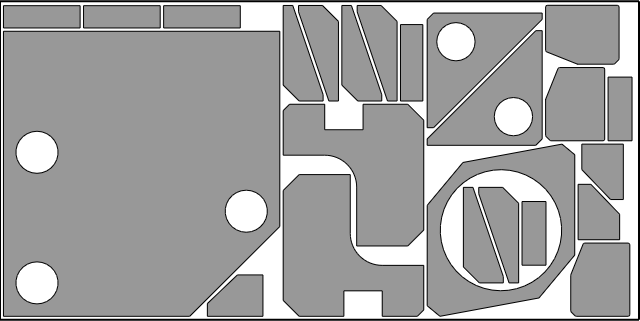
\includegraphics[width=0.9\textwidth]{nesting.png}
  \caption{Пример раскроя листа $2000 \times 1000$ мм с заданным минимальным расстоянием между деталями 10 мм}
  \label{nesting}
  \end{center}
\end{figure}

Раскройная карта
на рис.~\ref{nesting}
получена с помощью подсистемы автоматического раскроя
\textit{CAD/CAM}
системы <<Сириус>>.

Предположим, что для вырезки деталей было использовано
$K$
сегментов резки
$S_k=M_kM^*_k; k \in \overline{1,K}$.
Тогда маршрут резки деталей можно определить
в терминах сегментов резки как кортеж
\begin{equation}
  ROUTE = \left<
    M_0, M_1, S_1, M_1^*, M_2, S_2, M_2^*, \,\dots, M_K, S_K, M_K^*,
    i_1, i_2, \,\dots, i_K
  \right>
  ,
  \label{tuple}
\end{equation}
где
$M_0$
-- начальная точка положения инструмента,
$i_1, i_2, \,\dots, i_K$
– последовательность, в которой вырезаются используемые сегменты резки
$S_1, S_2, \,\dots, S_K$.
Линейное перемещение инструмента на холостом ходу
между точкой выключения инструмента и следующей точкой врезки
однозначно определяется этой последовательностью.
Если применить комбинаторную терминологию,
то последовательность однозначно задается перестановкой порядка
$K$,
т. е. упорядоченным набором натуральных чисел от $1$ до $K$
(биекцией на множестве $\overline{1,K}$),
которая числу
$k \in \overline{1,K}$
ставит в соответствие элемент
$i_k$ из набора.
Отметим, что термин <<маршрут резки>> является
общепринятым технологическим понятием.
В главах 3 -- 5 при описании математических моделей оптимизации
маршрута резки мы будем использовать термин <<маршрут>>
применительно к перестановке
$i_1, i_2, \,\dots, i_K$,
что, в свою очередь, соответствует устоявшейся
терминологии в задаче о последовательном обходе мегаполисов.

На рис.~\ref{cutting}
показана схема одного из возможных маршрутов резки для примера,
приведенного на рис.~\ref{nesting}.

\begin{figure}[h]
  \begin{center}
  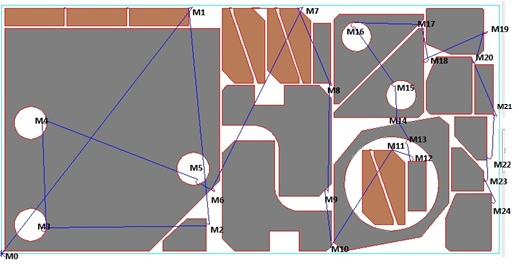
\includegraphics[width=0.9\textwidth]{cutting.png}
  \caption{Пример маршрута резки, содержащего 24 сегмента резки}
  \label{cutting}
  \end{center}
\end{figure}

Маршрут резки содержит 24 сегмента.
Для резки внешних контуров трех групп деталей
с точками врезки $M_1$
(три детали в группе),
$M_7$
(четыре детали в группе) и
$M_{11}$
была использована мультиконтурная резка
(указанные группы деталей выделены коричневым цветом).
Все остальные контуры вырезаны с применением стандартной техники резки.
Последовательность резки сегментов соответствует
номерам точек врезки $M_J$ ($J=1,2,\,\dots, 24$).
После вырезки последнего сегмента
возврат инструмента в начальную точку $M_0$
не программировался.

На приведенном рис.~\ref{cutting}
визуализация траектории инструмента
осуществляется точно по граничным контурам деталей,
а не по их эквидистантным контурам, хотя,
как отмечено выше,
траектория реза должна отстоять от
граничного контура на половину ширины реза.
Это связано с тем, что в большинстве
\textit{CAM}-систем
(\textit{Computer Aided Manufacturing})
программирование движения инструмента первоначально
осуществляется по граничным контурам деталей,
а вычисление реальной траектории производится
либо непосредственно самой системой ЧПУ,
либо специальной программой-постпроцессором,
предназначенной для конвертирования информации о
маршруте резки из внутреннего формата системы в
формат команд конкретного технологического оборудования с ЧПУ.
В этом случае величину припуска на рез
устанавливает оператор на станке перед запуском
управляющей программы резки.

В дальнейшем без ограничения общности мы будем полагать,
что траектория инструмента в маршруте резки $ROUTE$
программируется по граничным контурам,
и сегменты резки
$S_k=M_kM^*_k; k \in \overline{1,K}$
содержат все граничные контуры деталей
$C_1, C_2, \,\dots, C_N$,
т. е.
$$
\bigcup_{j=1}^N C_j \subset \bigcup_{k=1}^K S_k
$$

Соответственно, все точки входа в эквидистантный контур
(и выхода из эквидистантного контура)
также лежат на граничных контурах,
см. рис.~\ref{standard-cutting}.

На рис.~\ref{control-program}
показан фрагмент управляющей программы
($G$-кода) для машины листовой газовой резки
типа <<Комета>> с системой ЧПУ 2Р32М.

\begin{figure}
\begin{multicols}{3}

  \%УП\_2Р32М\_01
  N1G91 \\
  N2G00X7662Y9909F6000 \\
  N3M70T1 \\
  N4M71T1 \\
  N5G01X-141Y-48F460 \\
  N6X-2400  \\
  N7X-40  \\
  N8X-67  \\
  N9X-2400  \\
  N10X-40 \\
  N11X-67 \\
  N12X-2400 \\
  N13Y-700  \\
  N14X2400  \\
  N15Y700 \\
  N16Y40  \\
  N17X107Y-40 \\
  N18Y-700  \\
  N19X2400  \\
  N20Y700 \\
  N21Y40  \\
  N22X107Y-40 \\
  N23Y-700  \\
  N24X2400  \\
  N25Y700 \\
  N26Y40  \\
  N27M74T1  \\
  N28G00X817Y-8745F6000 \\
  N29M71T1  \\
  N30G03X-108Y0I-54J0F460 \\
  N31G01Y-1048  \\
  N32X-1740 \\
  N33Y400 \\
  N34X940Y900 \\
  N35X800 \\
  N36Y-252  \\
  N37X20Y-30  \\
  … \\
  N314M71T1 \\
  N315G02X-130Y0I-65J0F460  \\
  N316G01Y267 \\
  N317G03X-50Y50I-50J0  \\
  N318G01X-1366 \\
  N319G03X-46Y-31I0J-50 \\
  N320G01X-384Y-960 \\
  N321G03X-4Y-19I46J-19 \\
  N322G01Y-1120 \\
  N323G03X14Y-35I50J0 \\
  N324G01X122Y-121  \\
  N325G03X37Y-14I35J35  \\
  N326G01X1627Y-1 \\
  N327G03X50Y50I0J50  \\
  N328G01Y1933  \\
  N329X20Y30  \\
  N330M74T1 \\
  N331M75T1 \\
  N332M02 \\
  M30
\end{multicols}
\caption{Фрагмент УП для машины листовой резки <<Комета>> с ЧПУ 2Р32М }
\label{control-program}
\end{figure}

Программа сгенерирована на основе маршрута резки
(спроектированного в интерактивном режиме в
\textit{CAD/CAM} системе <<Сириус>>
и показанного на рис.~\ref{cutting})
соответствующим постпроцессором со
следующими числовыми параметрами резки:
\begin{itemize}
  \item	число строк в УП – 333;
  \item	количество точек врезки (пробивки листа) – 24;
  \item	путь инструмента на рабочей скорости – 27,36 м;
  \item	путь инструмента на быстром (холостом) ходу – 8,39 м;
  \item	время движения на рабочей скорости – 62,04 мин;
  \item	время движения на быстром (холостом) ходу – 1,64 мин;
  \item	общее время резки: 63,68 мин.
\end{itemize}

В зависимости от выбранного маршрута резки
числовые параметры резки могут существенно различаться.
Таким образом, при разработке управляющих программ
для машин фигурной листовой резки с ЧПУ возникают
различные задачи оптимизации маршрута инструмента.
В качестве критерия оптимизации (целевой функции)
в этих задачах чаще всего рассматривается общее время резки.
При термической и гидроабразивной резке для сформированного
маршрута резки общее время резки
$T_{cut}$
рассчитывается по следующей формуле:
\begin{equation}
  T_{cut} = \frac{L_{on}}{V_{on}} + \frac{L_{off}}{V_{off}} +N_{pt} \cdot t_{pt}
  ,
  \label{cutting-time}
\end{equation}
где
$L_{on}$ -- длина реза с включенным режущим инструментом;
$V_{on}$ -- скорость рабочего хода режущего инструмента;
$L_{off}$ -- длина переходов с выключенным режущим инструментом (холостой ход);
$V_{off}$ -- скорость холостого хода;
$N_{pt}$ -- количество точек врезки;
$t_{pt}$ -- время, затрачиваемое на одну точку врезки.
При этом подразумевается,
что получаемое в результате врезки отверстие
расположено внутри материала листа.
Однако при резке заготовок, как отмечалось,
могут быть использованы и другие типы врезки,
что приводит к изменению времени врезки
$t_{pt}$
в этих случаях.
Если при резке деталей было использовано несколько типов врезки,
то формула~(\ref{cutting-time}) запишется в более общем виде:
\begin{equation}
  T_{cut} = \frac{L_{on}}{V_{on}} + \frac{L_{off}}{V_{off}} +
  \sum_{j=1}^p N_{pt}^j \cdot t_{pt}^j
  ,
  \label{cutting-time-multi}
\end{equation}
где
$p$ -- число использованных типов врезки,
$N_{pt}^j$ -- количество точек врезки типа $j$;
$t_{pt}^j$ -- время, затрачиваемое на одну точку врезки типа $j$.

И в (\ref{cutting-time})
и в (\ref{cutting-time-multi})
значение скорости холостого хода инструмента
$V_{off}$ -- константа,
определяемая техническими характеристиками
используемого технологического оборудования.
Значение скорости рабочего хода инструмента
$V_{on}$
программируется при разработке управляющей программы
в соответствии с используемой технологией резки
и параметрами листового материала
(марка материала и толщина).
Предполагается, что заданная величина
$V_{on}$  в (\ref{cutting-time}) и в (\ref{cutting-time-multi})
также является константой,
однако на практике фактическая скорость резки
может меняться в зависимости от различных технологических факторов,
а также характеристик спроектированной управляющей программы.
Это диктует необходимость проведения исследований для
определения поправочного коэффициента для величины
$V_{on}$.
В \ref{sect:1.4}
приведены результаты такого рода исследований
применительно к машине лазерной резки с ЧПУ
\textit{ByStar 3015}
для листового материала
\textit{АМг3М} толщиной от 1,5 до 5 мм.

Важнейшей экономической характеристикой качества
разработанной управляющей программы является стоимость
(себестоимость) резки деталей на машине с ЧПУ.
Это сложный интегрированный показатель,
который включает в себя произведенные во время
резки затраты на электроэнергию и расходные материалы,
на обслуживание машины с ЧПУ,
а также другие эксплуатационные затраты.
Отметим, что стоимость резки не всегда
пропорциональна времени резки,
поскольку зависит еще и от различных режимов резки.
По аналогии с формулой времени резки (\ref{cutting-time})
показатель стоимости резки можно определить по следующей формуле:
\begin{equation}
  F_{cost}=
  L_{on} \cdot C_{on} +
  L_{off} \cdot C_{off} +
  N_{pt} \cdot C_{pt}
  ,
  \label{cutting-cost}
\end{equation}
где
$C_{on}$ -- стоимость единицы пути с включенным режущим инструментом;
$C_{off}$ -- стоимость единицы пути с выключенным режущим инструментом;
$C_{pt}$ -- стоимость одной точки врезки,
а $L_{on}, L_{off}, N_{pt}$
имеют тот же смысл, что и в формуле~(\ref{cutting-time}).
При этом $C_{on}, C_{off}, C_{pt}$ --
величины, зависящие от типа машины с ЧПУ,
технологии резки, используемой скорости рабочего хода инструмента,
толщины и марки материала.
Функциональная зависимость
$C_{on}, C_{off}, C_{pt}$
от перечисленных параметров
может задаваться либо табличными функциями,
либо аналитически.
При этом абсолютные значения этих величин
на российских предприятиях, использующих машины с ЧПУ,
определяются экономическими службами с учетом многих факторов
и могут существенно различаться на разных предприятиях.
Зачастую стоимость резки вообще не учитывается
в раскройно-заготовительном производстве,
либо рассчитывается на основании специальных нормативов,
не зависящих от величин
$L_{on}, L_{off}, N_{pt}$.

Очевидно, что необходимость расчета стоимости резки
для каждой управляющей программы резки возникает на предприятиях,
оказывающих услуги сторонним организациям по резке материала.
Однако и на многих таких предприятиях для определения
стоимости резки учитывается только длина рабочего хода инструмента
$L_{on}$,
которая принимается равной суммарному периметру граничных контуров вырезаемых деталей
$C_1, C_2, \,\dots, C_N$,
что, естественно, приводит к неадекватной оценке эффективности процесса резки.
В дальнейшем при оптимизации стоимостных параметров резки
мы будем применять теоретически обоснованный способ определения
показателя стоимости резки, задаваемый формулой (\ref{cutting-cost}).

На рис.~\ref{cost} представлен расчет стоимости резки
$F_{cost}$
для рассматриваемого примера при резке деталей на машине газовой резки.
Значения величин
$C_{on}, C_{off}, C_{pt}$
взяты из таблицы, используемой для расчета себестоимости фигурной
листовой резки на одном из предприятий Свердловской области.

\begin{figure}[h]
  \begin{center}
  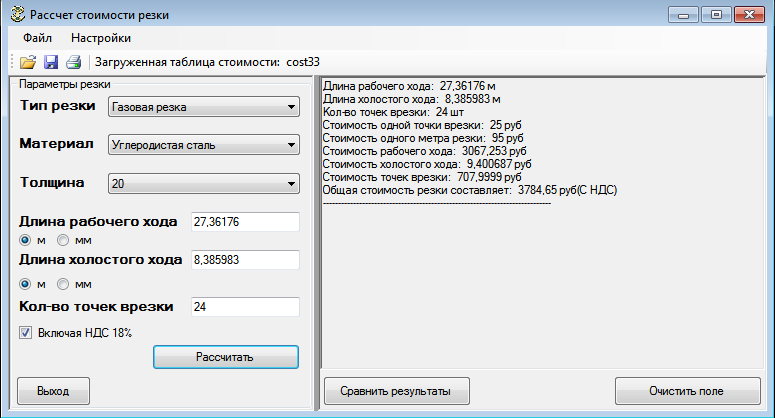
\includegraphics[width=0.95\textwidth]{cost.png}
  \caption{
    Пример расчета стоимости резки $F_{cost}$
    при резке деталей из~углеродистой стали
    толщины 20~мм на~машине газовой резки}
  \label{cost}
  \end{center}
\end{figure}

Следует отметить,
что задача правильного определения величин
$C_{on}$, $C_{off}$, $C_{pt}$
для конкретного технологического оборудования
и конкретного материала сама по себе является малоисследованной проблемой.
В \ref{sect:1.4}
приведены результаты исследования,
позволяющего точно вычислять себестоимость
лазерной резки применительно для машины с ЧПУ
\textit{ByStar3015}
при резке углеродистой и нержавеющей
стали различных толщин
(на примере Ст10кп и 12Х18Н10Т),
а также при резке алюминия и его сплавов
(на примере \textit{Амг3М}).

В случае использования нескольких типов врезки формула~(\ref{cutting-cost}) примет вид:
\begin{equation}
  F_{cost}=
  L_{on} \cdot C_{on} +
  L_{off} \cdot C_{off} +
  \sum_{j=1}^p N_{pt}^j \cdot C_{pt}^j
  ,
  \label{cutting-cost-multi}
\end{equation}
где $C_{pt}^j$ -- стоимость одной точки врезки типа $j$.

Как легко заметить,
значения целевых функций (\ref{cutting-time}) -- (\ref{cutting-cost-multi})
однозначно определяются маршрутом резки,
задаваемым кортежем (\ref{tuple}),
поскольку геометрия сегментов резки
$S_1, S_2, \,\dots, S_K$
позволяет вычислить длину рабочего хода инструмента  $L_{on}$,
а координаты точек
$M_0$, $M_1$, $M_1^*$, $M_2$, $M_2^*$, \,\dots, $M_K$, $M_K^*$
и перестановка
$i_1$, $i_2$, \,\dots, $i_K$
(последовательность, в которой вырезаются используемые сегменты резки)
задают набор холостых перемещений инструмента,
который определяет суммарную длину холостого хода
$L_{off}$.

Таким образом, сформулированные задачи оптимизации
маршрута инструмента для машин фигурной листовой резки с ЧПУ
можно представить в самом общем виде
как задачу минимизации некоторой числовой функции $F$,
заданной на множестве $G$ допустимых кортежей $ROUTE$,
т. е.
\begin{equation}
  F(ROUTE) \to \min_{ROUTE \in G}
  .
  \label{problem-statement}
\end{equation}

Поскольку элементы кортежа содержат
(помимо последовательности резки
$i_1, i_2, \,\dots, i_K$,
выбираемой из дискретного множества перестановок)
точки врезки и точки выключения инструмента
$M_kM_k^*, k \in \overline{1,K}$,
которые, в свою очередь,
могут быть выбраны из континуальных подмножеств евклидовой плоскости
$\mathbb R \times \mathbb R$,
даже в случае наложения существенных ограничений
на возможность выбора допустимых сегментов
$S_k$
оптимизационная задача (\ref{problem-statement})
может быть отнесена к классу очень сложных задач
непрерывно-дискретной оптимизации.
Некоторые вопросы формирования допустимых сегментов резки мы рассмотрим в части 2
настоящей монографии при математической формализации задачи (\ref{problem-statement})
и ее сведении к задаче о последовательном обходе мегаполисов.
В следующем параграфе мы сформулируем основные ограничения
на допустимые значения элементов последовательности резки
$i_1, i_2, \dots i_K$
и на значения
$M_kM_k^*, k \in \overline{1,K}$,
вызванные особенностями технологии листовой резки на машинах с ЧПУ.

% !TeX root = ..

%!!! Проверить в финальном варианте !!!
%\newpage
\section{
  Технологические ограничения параметров маршрута инструмента
  машин листовой резки с~ЧПУ
}
\label{sect:1.3}
\setcounter{equation}{0}

% !TeX root = ../mat_mod2.tex

\subsection{\protect\raggedright
  Ограничения координат точек врезки и точек выключения инструмента,
  обусловленные деформацией материала при врезке
}
\label{sect:1.3.1}

Этот тип ограничений связан с тем,
что для соблюдения технологии врезки любая точка врезки
$M_k$
должна лежать (как отмечалось выше)
на некотором ненулевом расстоянии от контура детали,
по которому движется инструмент.
При этом координаты точки врезки должны,
естественно, находиться вне областей,
занимаемых геометрическими образами других деталей с учетом припуска на рез.
Величины необходимых минимально допустимых расстояний
от контуров детали до точек врезки и точек выключения
инструмента определяются различными технологическими параметрами.
Другими словами, этот тип ограничений носит геометрический характер
и определяет геометрические области на раскройной карте,
в которых допустимо задавать точки врезки для формирования сегментов резки.

Для общей формализации этих ограничений обозначим через
$E_j^d$ эквидистанты замкнутых контуров $C_j$,
удаленные от них на величину $d$,
а через
$P_j^d$ двумерные геометрические объекты
(замкнутые точечные множества),
ограниченные этими эквидистантами:
$E_j^d = \partial P_j^d$,
$P_j^d \subset \mathbb R \times \mathbb R$.
При этом будем полагать,
что для внешних контуров деталей
$E_j^d$
является внешней эквидистантой,
а для внутренних -- внутренней.
Пусть $ОUT$ -- конечное множество индексов внешних контуров деталей,
а $IN$ -- соответственно множество индексов внутренних контуров.
Обозначим  размерность этих множеств соответственно $l$ и $s$,
т. е.
$OUT = \{j_1, j_2, \,\dots, j_l\};
IN = \{q_1, q_2, \,\dots, q_s\}$
$(OUT \subseteq \overline{1,N};
IN \subset \overline{1,N})$.
Заметим, что если $l=N$
(все контуры являются внешними), то
$IN = \varnothing$
$(s = 0)$.
Пусть $d1$ -- минимально допустимое расстояние от контуров деталей до точек врезки,
тогда выбранные точки врезки для каждого сегмента резки должны удовлетворять следующим условиям:
\begin{equation}
  \forall k \in \overline{1,K}:
  M_k \in G_M,
  \text{где}\:
  G_M = \big(B \setminus \bigcup_{j\in OUT} P_j^{d1} \big)
  \cup
  \big( \bigcup_{q\in IN}P_q^{d1} \big)
  .
  \label{pierce-constraint}
\end{equation}

Как мы уже отмечали,
минимально допустимое расстояние от граничных контуров деталей
до точек врезки,
задаваемых на границе листа,
или подготовленных предварительно механическим способом,
может быть несколько меньше,
чем до точек врезки, получаемым стандартным <<прожиганием>> (пробивкой) материала листа.
Для таких особых точек врезки область $G_M$,
задаваемая условием (\ref{pierce-constraint}),
может быть расширена.
Это условие является необходимым, но не достаточным,
и для конкретных задач могут возникать дополнительные ограничения,
обусловленные технологическими особенностями резки,
о которых пойдет речь ниже.
В этих случаях, наоборот, область $G_M$
может быть существенно сокращена.

Аналогичное условию (\ref{pierce-constraint})
ограничение справедливо и для точек выключения инструмента:
\begin{equation}
  \forall k \in \overline{1,K}:
  M_k^* \in G_{M^*},
  \text{где}\:
  G_{M^*} = \big(B \setminus \bigcup_{j\in OUT} P_j^{d2} \big)
	\cup
  \big( \bigcup_{q\in IN}P_q^{d2} \big)
  ,
  \label{tool-off-constraint}
\end{equation}
где $d2$ -- минимально допустимое расстояние
от контуров деталей до точек выключения инструмента,
которое чаще всего меньше $d1$
и может, как отмечалось, быть и нулевым.

На рис.~\ref{pierce-area}
указаны геометрические области листа,
допустимые для определения точек врезки при программировании резки
внешних граничных контуров деталей,
обозначенных на рисунке
\textit{1,2} и \textit{3}
и внутреннего граничного контура
\textit{4}.
При этом минимально допустимое расстояние $d1$
от граничных контуров
\textit{1 -- 4} до возможных точек врезки,
установленное пользователем
\textit{CAM}-системы, равно 9,5 мм.

\begin{figure}[h]
  \begin{center}
  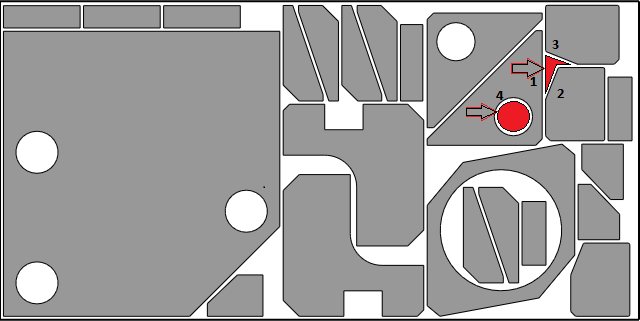
\includegraphics[width=0.9\textwidth]{pierce-area.png}
  \caption{
    Пример двух геометрических областей на раскройной карте
    (указаны~стрелками),
    допустимых для задания точек врезки
  }
  \label{pierce-area}
  \end{center}
\end{figure}

% !TeX root = ..

\subsection{
  Условие предшествования
}
\label{sect:1.3.2}

Это условие накладывает ограничения на порядок вырезки сегментов
$ I = (i_1, i_2, \,\dots, i_K)$.
Ограничения на порядок их резки обусловлены особенностями
технологии и оборудования листовой резки с ЧПУ,
которые не позволяют после вырезки внешнего контура точно
позиционировать инструмент для вырезки внутренних контуров,
поскольку деталь после вырезки внешнего контура может
изменить свое положение на раскройном столе.
Это вызвано тем, что после вырезки внешнего контура
вырезанная деталь <<теряет>> связь с листом,
а для многих типов раскройных столов эта деталь
может даже изменить свое положение относительно плоскости листа
(упасть между статическими конструкциями раскройного стола).
При выборе последовательности контуров
необходимо придерживаться следующих правил.

{\it Правило 1}.
Если внешний контур имеет один или более внутренних контуров,
которые представляют собой границы отверстий в деталях,
то прежде, чем будет начата вырезка внешнего контура,
должны быть вырезаны все внутренние контуры.

{\it Правило 2}.
Если внутренний контур детали на раскройной карте
содержит внешний контур/контуры другой детали,
то сначала должна быть вырезана эта другая деталь
с соблюдением {\it Правила 1}.

Перечисленные правила и называются условием предшествования для перестановки
$ I = (i_1, i_2, \,\dots, i_K)$.
В терминах ее элементов условие означает следующее:
\begin{itemize}
  \item
  если в перестановке
  $ I = (i_1, i_2, \,\dots, i_K)$
  сегмент $i_k$
  содержит внешний контур,
  то все соответствующие внутренние контуры должны содержаться в сегментах,
  предшествующих сегменту $i_k$
  в перестановке;
  \item
  если в перестановке
  $ I = (i_1, i_2, \,\dots, i_K)$
  сегмент $i_k$
  содержит  внутренний контур,
  который на раскройной карте содержит внутри внешний контур,
  соответствующий другому объекту
  $A_l$
  $(l=1,2, \,\dots, n)$,
  то этот внешний контур должен быть вырезан в сегментах,
  предшествующих сегменту $i_k$ в перестановке $I$.
\end{itemize}

Рис.~\ref{precedence}
иллюстрирует условие предшествования
при формировании маршрута резки для деталей,
содержащих внутренние контуры
(первое правило),
а также деталей,
расположенных в отверстиях
больших деталей
(второе правило).

В соответствии с условиями предшествования резка контуров,
ограничивающих цветные области для четырех деталей на
рис.~\ref{precedence},
должна осуществляться в следующей последовательности:
\begin{enumerate}
  \item желтый, красный, синий, серый;
  \item	красный, синий, серый;
  \item	желтый, серый;
  \item желтый, серый.
\end{enumerate}

\begin{figure}[H]
  \centering
  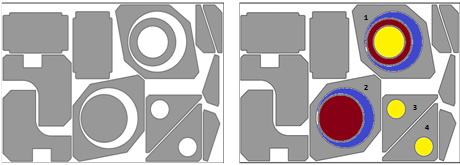
\includegraphics[width=0.9\textwidth]{precedence.png}
  \caption{
    Пример раскройной карты деталей, содержащих внутренние контуры
  }
  \label{precedence}
\end{figure}

Условия предшествования и ограничения координат точек врезки
и точки выключения инструмента,
обусловленные деформацией материала при врезке,
имеют статический характер,
т. е. однозначно определяются спроектированной раскройной картой,
используемым для резки технологическим оборудованием
и свойствами раскраиваемого материала.
В терминах маршрута резки $ROUTE$
и его параметров
$M_0$, $M_1$, $S_1$, $M_1^*$, $M_2$, $S_2$, $M_2^*$, \,\dots, $M_K$, $S_K$, $M_K^*$,
$i_1$, $i_2$, \,\dots, $i_K$
первое технологическое ограничение 
однозначно определяет допустимые геометрические области
$G_M$
и
$G_{M^*}$
для выбора точек врезки и точек выключения инструмента,
второе а технологическое ограничение 
накладывает запрет на некоторые значения перестановки
$ I = (i_1, i_2, \,\dots, i_K)$
при формировании порядка резки сегментов.
При этом сформулированные требования не зависят от задаваемых параметров кортежа
$ROUTE$.

В отличие от этих двух технологических ограничений
следующий тип технологических требований устанавливает
дополнительные ограничения на выбор точки врезки и выбор
порядка резки сегментов на каждом шаге формирования маршрута резки
(т. е. при определении параметров очередного выбираемого сегмента)
в зависимости от того, какие параметры маршрута резки были выбраны на предыдущих шагах.
Этот тип ограничений обусловлен геометрическими
искажениями материала при термической резке деталей.

% !TeX root = ..

\subsection{
  Эвристические правила термической резки заготовок
  из~листовых материалов
}
\label{sect:133}

Термические воздействия на вырезаемые заготовки можно подразделить на два типа\footnote{
  Сформулированные в \ref{sect:133}
  правила разработаны сотрудниками ОАО~<<Уралхиммаш>>
  В.~И.~Кротовым и А.~Д.~Гуртовенко на основе опыта
  резки листовых материалов на машинах термической резки с~ЧПУ
  в котельно-заготовительном комплексе предприятия в~1992~г.
}:

\begin{itemize}
\item
общие изменения геометрических размеров заготовки (уменьшение)
вследствие ее вырезания из нагретой части материала;
\item
изменение геометрической формы заготовок
(изменение радиусов у секторов,
отклонения от прямолинейности у прямоугольных деталей) и др.
Чем больше геометрические размеры заготовки,
тем больше изменения.
Наиболее  подвержены изменениям узкие длинные заготовки.
\end{itemize}

В табл.~\ref{thermal-classification}
на стр.~\pageref{thermal-classification}
приведена типология некоторых видов заготовок
по признаку подверженности термическим деформациям.
В качестве основных геометрических характеристик
классификации заготовок использованы габаритные размеры заготовок
($A$ -- габаритная длина,
$B$ -- габаритная ширина).
Приведенные в табл.~\ref{thermal-classification}
типы заготовок относятся,
в основном, к номенклатуре машиностроительных предприятий,
но широко используются также в раскройно-заготовительном производстве
других отраслей промышленности.

В зависимости от термических характеристик заготовок
и~требований к~их~точности выбирается оборудование,
способ и последовательность резки.
Например, величина удельного тепловыделения --
наибольшая при газокислородной резке,
поэтому имеет смысл тонкие листы из углеродистых и
низколегированных сталей резать плазменно-дуговым способом,
дающим попутно больший выигрыш в производительности.
Металлы, обладающие более высокой теплопроводностью,
менее склонны к термическим деформациям.
Термообработка листового проката уменьшает
тепловые деформации материала и наоборот,
необработанный лист более склонен к термическим деформациям,
т. к. в нем присутствуют высокие внутренние  напряжения,
которые накладываются на усилия, возникающие от  нагрева при резке.

\begin{table}[p]
  \caption{
    Классификация заготовок по признаку подверженности термическим~деформациям
    }
  \label{thermal-classification}
  \begin{tabular}{ p{0.3\textwidth} | p{0.3\textwidth} | p{0.3\textwidth} }
  \hline
  Термическая характеристика заготовки
    & Описание заготовки
    & Геометрические характеристики заготовки \\
  \hline
  \hline
  Заготовки, подверженные термическим деформациям изгиба
    & Полосы, узкие обечайки, секторы
    &	$B<100 \text{ мм}, A>5B$ $100<B<250, A>8B$ \\
  \hline
    Заготовки, подверженные термическим деформациям изгиба и изменением длины
    & Длинномерные и узкие полосы и обечайки, длинномерные секторы больших радиусов ($R>200$ мм)
    & $B <100 \text{ мм}, A>10B$ $100<B< 300, A \hm >15B$ \\
  \hline
    Заготовки, не подверженные термическим деформациям
    & Фланцы, заглушки, диски, косынки, ребра, стенки, широкие сегменты и обечайки
    & $A/B < 5$ \\
  \hline
    Заготовки, подверженные оплавлению и загрязнению при резке
    & Малогабаритные косынки, планки, ребра
    & $ A, B <200 \text{ мм}$ \\
  \hline
    Заготовки, вырезаемые с большим удельным тепловыделением
    & Полосы, обечайки, секторы со скосами кромок под сварку
    & $ A>300 \text{ мм}, B \hm >150 \text{ мм}$ \\
  \hline
  \end{tabular}
\end{table}

На величину термических деформаций оказывают влияние:
\begin{itemize}
\item	тип резки (газовая, плазменная, лазерная);
\item	марка материала (его теплопроводность);
\item	состояние поставки металла (наличие внутренних напряжений), его термообработка;
\item	толщина металла;
\item	выбор порядка резки заготовок;
\item	выбор точек врезки для каждого контура;
\item	направление обхода контура (по/против часовой стрелки).
\end{itemize}

При работе в интерактивном режиме в
\textit{CAM}-системе
пользователь может сам определять контуры или их части
для формирования сегментов резки,
выбирать порядок резки сегментов и координаты точек врезки
в нужном месте посредством курсора <<мыши>>.
Автоматический режим предполагает наличие в
\textit{CAM}-системе
соответствующего алгоритма определения маршрута резки
$ROUTE$
с соблюдением необходимых технологических требований.
Сформулируем наиболее важные из технологических требований резки,
обусловленные наличием термических деформаций материала.
Прежде всего, введем понятия правил
<<жесткости заготовки>> и <<жесткости материала>>.

\paragraph*{Правило <<жесткости заготовки>> (<<жесткости детали>>)}

касается выбора точек врезки
$M_k, k \in \overline{1,K}$
в маршруте резки  $ROUTE$,
а также выбора направления резки контуров деталей.
Оно заключается в том, что при резке контура точка
врезки и направление резки контура выбираются таким образом,
чтобы сначала вырезались участки контура,
расположенные в непосредственной близости к границе материала,
либо к границе вырезанной области,
а завершение резки происходило по участку контура,
граничащего с <<жесткой>> (не вырезанной) частью области.

Поясним правило <<жесткости заготовки>> на примере.
На рис.~\ref{part-hardness}
показаны три заготовки
и~девять выбранных возможных точек врезки.

Предположим, что мы начинаем резку с нижней заготовки
и выбираем одну из первых четырех точек врезки
(\textit{1 -- 4}).
Точка \textit{2} является недопустимой для врезки,
поскольку при завершении резки не остается
<<жесткого>> участка не вырезанной области в материале,
и заготовка (еще до завершения резки контура)
начнет перемещаться относительно материала.
Кроме этого, заготовка будет получать максимальное
нагревание из-за малой площади остатка в области завершения резки.
Все это, в конечном итоге,
приведет к искажению геометрических размеров заготовки.

\begin{figure}[H]
  \centering
  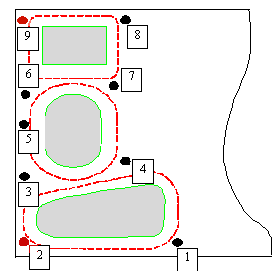
\includegraphics[width=0.5\textwidth]{part-hardness.png}
  \caption{
    Пример выбора точек врезки
  }
  \label{part-hardness}
\end{figure}

Точки
\textit{1,3} и \textit{4}
являются допустимыми для врезки,
однако при выборе точки врезки {\it 1} резка контура
должна производиться по часовой стрелке,
а при выборе точки {\it 3} - против.
Для точки {\it 4} -- направление реза не является существенным.
При резке следующей (средней) заготовки
допустимы точки врезки {\it 4,6} или {\it 7}.
Для точки {\it 4} правило <<жесткости заготовки>>
предполагает движение резака по часовой стрелке,
а для точки {\it 6} – против часовой стрелки.

И, наконец, при резке верхней заготовки
допустимы точки врезки {\it 7} или {\it 8}.
Выбор точки врезки {\it 7} диктует необходимость
движения резака по часовой стрелке,
а в случае выбора точки {\it 8} – против часовой стрелки.

Таким образом, правило <<жесткости заготовок>>
существенно ограничивает свободу выбора точек
врезки и направлений обхода контура.
В частности для данного примера,
если все контуры вырезаются по часовой стрелке,
то набор точек врезки {\it 1, 4, 7}
является наиболее предпочтительным,
а если против часовой стрелки, то -- {\it 4, 7, 8}
(или {\it 4, 6, 8}).
Понятно, что строгая формализация процедуры
выбора представляется затруднительной,
и~остальные допустимые варианты также не приведут
к~критическим изменениям в геометрии заготовок,
но интуитивно ясно, что предлагаемые три варианта
несколько уменьшат тепловые деформации по сравнению
с~другими допустимыми вариантами.

Важно отметить,
что при изменении порядка вырезки заготовок
(например, в последовательности сверху вниз)
изменится и набор допустимых точек врезки и направлений реза.

Функция определения допустимых
(как с точки зрения геометрических характеристик,
так и с точки зрения технологических требований резки)
точек врезки является важнейшей функцией
{\it CAM}-системы
при автоматическом режиме формирования УП.

\paragraph*{Правило <<жесткости материала>> (<<жесткости листа>>)}

определяет допустимый порядок
(последовательность)
$i_1, i_2, \,\dots, i_k$,
в котором вырезаются используемые сегменты резки
$S_1, S_2, \,\dots, S_K$.
Фактически это правило включает в себя несколько
эмпирических условий.

Рис.~\ref{list-hardness}
на стр.~\pageref{list-hardness}
демонстрирует четыре условия выбора стороны материала,
с которой следует начинать процесс термической резки.
Условие а) рекомендует начинать процесс резки с узкой стороны листа (материала).
Условия б), в) и г) уточняют,
какую из узких сторон выбрать.
Алгоритм выбора заключается в следующем.

\begin{enumerate}
  \item
  Сначала определяем,
  есть ли среди заготовок длинномерные детали
  (длинномерной деталью в соответствии с~табл.~\ref{thermal-classification}
  на стр.~\pageref{thermal-classification}
  будем называть заготовки, у которых один из габаритов больше другого не менее,
  чем в 10 раз).
  Если эти заготовки расположены вблизи
  узкой границы материала,
  то процесс резки следует начинать с них
  (рис.~\ref{list-hardness}, б),
  так как именно такого рода заготовки
  подвержены максимальным тепловым деформациям.
  \item
  Затем определяем,
  есть ли на материале крупный отход.
  При наличии такого отхода с одной из сторон
  процесс резки следует начать с противоположной стороны,
  поскольку аккумулирующееся в материале в~процессе резки
  тепло в конечной стадии резки должно быть
  несколько скомпенсировано <<жестким>> остатком
  (рис.~\ref{list-hardness}, в).
  \item
  И наконец,
  если на материале нет крупного отхода,
  резку следует начинать с той стороны,
  где суммарные тепловыделения от резки больше
  (больше мелких деталей, либо больше суммарный периметр реза),
  см. рис.~\ref{list-hardness}, г.
\end{enumerate}

\begin{figure}[H]
  \centering
  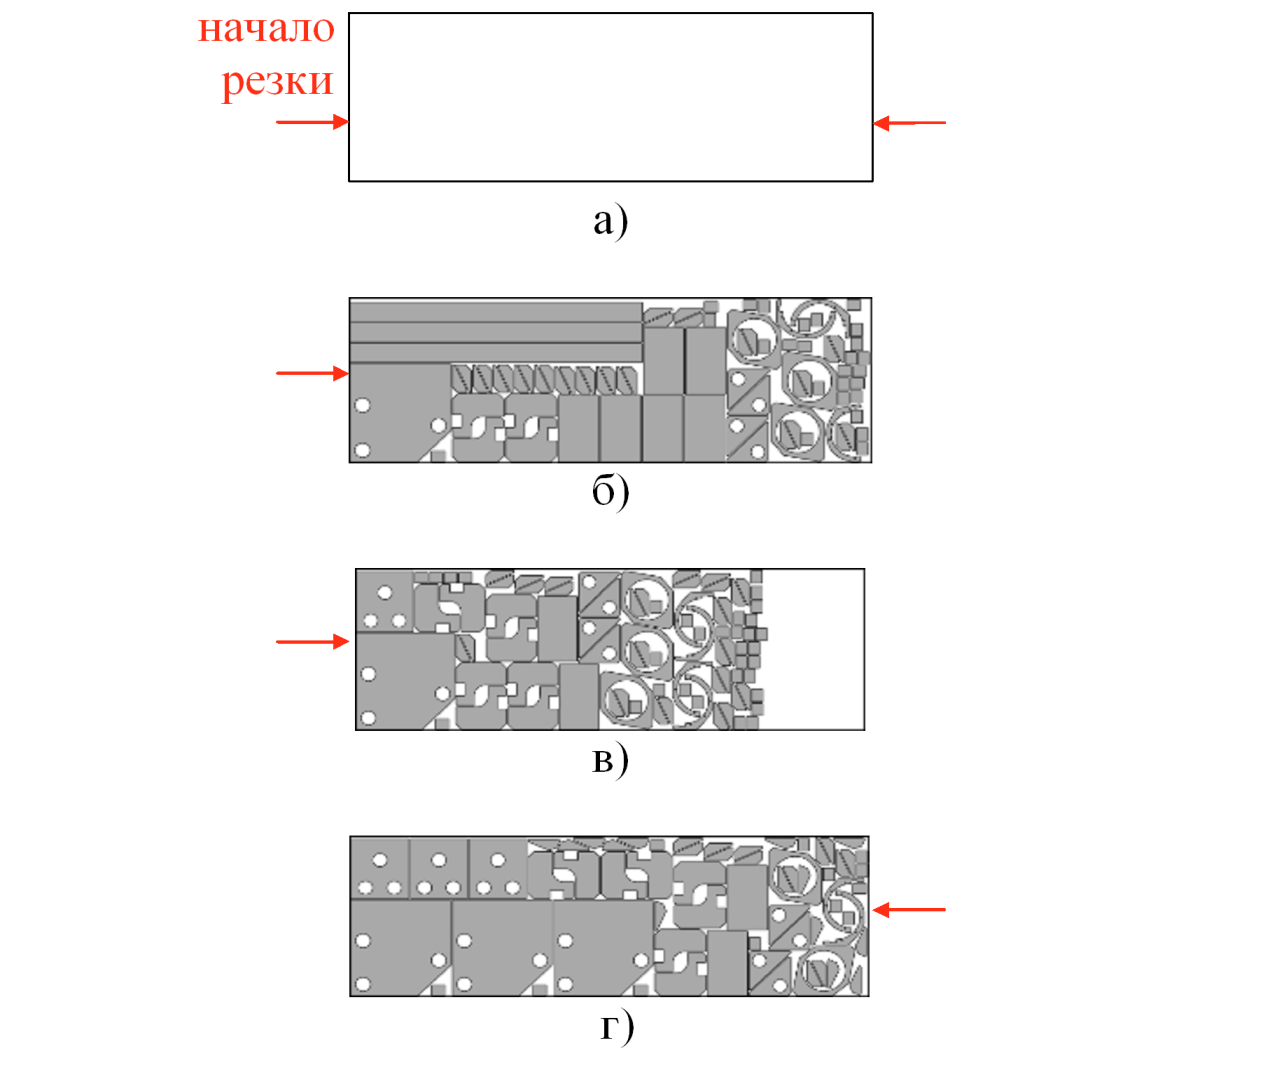
\includegraphics[width=0.9\textwidth]{list-hardness.png}
  \caption{
    Правила выбора начальной стороны материала
  }
  \label{list-hardness}
\end{figure}

Еще два условия <<жесткости>> заключаются в том,
что при выборе последовательности вырезаемых заготовок
на материале не должно оставаться узких полос и <<островов>>,
содержащих невырезанные заготовки
(рис.~\ref{island}).

Для того чтобы обеспечить все условия <<жесткости материала>>,
следует предварительно разбить всю область резки на некоторые <<зоны>>
и затем процесс резки заготовок осуществлять
в этих зонах последовательно по возрастанию номеров зон,
т. е. область размещения $B$ разбивается на подобласти
\begin{equation}
  \label{eq:cutting-zones}
  B_j = \bigcup_{r=1}^l \Omega_r
  ,
\end{equation}
где $l$
-- количество выбранных зон для области $B$.
При этом формирование и нумерация зон
должна проводиться в соответствии со всеми условиями правила
<<жесткости материала>>
таким образом,
чтобы оставшаяся не вырезанная область
по своей геометрической форме приближалась к квадратной области.

\begin{figure}[H]
  \centering
  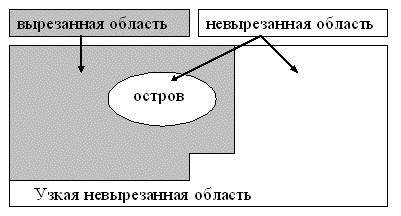
\includegraphics[width=0.6\textwidth]{island.png}
  \caption{
    Пример материала с недопустимыми не вырезанными областями
  }
  \label{island}
\end{figure}

Пример разбиения области термической резки на зоны
представлен на
рис.~\ref{zones}.
Цифрами {\it 1--12}
обозначены зоны,
выделенные на раскройной карте
в соответствии с (\ref{eq:cutting-zones}).

\begin{figure}[H]
  \centering
  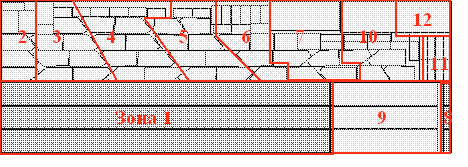
\includegraphics[width=0.9\textwidth]{zones.png}
  \caption{
    Пример формирования зон резки с учетом <<жесткости>> материала
  }
  \label{zones}
\end{figure}

Зоны {\it 1} и зона {\it 8},
выделенные на рисунке темно-серым цветом,
сформированы с учетом условия <<жесткости материала>>,
см. рис.~\ref{list-hardness}, б.

\subsubsection*{
  Заключительные замечания
}

В настоящее время в научных публикациях по теме монографии
наименее изученными остаются вопросы математической формализации ограничений,
связанных именно с технологическими требованиями термической резки.
Следует отметить, что, как показала практика,
правила <<жесткости заготовки>> и <<жесткости материала>>
целесообразно учитывать
не только при разработке управляющих программ для машин газовой,
плазменной и лазерной резки с ЧПУ,
но и при применении машин гидроабразивной фигурной листовой резки.
Этот факт свидетельствует о том,
что изменения геометрических характеристик материала
связаны не только с термическими деформациями,
но и с механическими трансформациями материала
при листовой резке заготовок на машинах с ЧПУ.
Рекламные заявления некоторых производителей
лазерных и гидроабразивных машин с ЧПУ о незначительных
деформациях вырезаемых заготовок при листовой фигурной
резке на данных типах технологического оборудования с ЧПУ
опровергаются практическими исследованиями.
Разумеется, лазерная и гидроабразивная технологии
порождают меньшие проблемы с тепловыми деформациями материала,
чем газовая и плазменная,
но не исключают полностью геометрические искажения формы заготовок при резке.

Если обозначить через
$ROUTE_\nu$
частичный маршрут резки первых $\nu$
сегментов
($\nu < K$)
$$
  ROUTE_\nu = \left<
    M_0, M_1, S_1, M_1^*, \,\dots, M_\nu, S_\nu, M_\nu^*,
    i_1, i_2, \,\dots, i_\nu
  \right>
  ,
$$
то правила <<жесткости заготовки>> и <<жесткости материала>>
при формировании допустимого маршрута
$ROUTE$,
помимо соблюдения условий предшествования для перестановки
$i_1, i_2, \,\dots, i_K$
и условий (\ref{pierce-constraint}) и (\ref{tool-off-constraint}),
формирует следующее дополнительное условие:
если
$ROUTE_\nu$ -- частичный маршрут,
допустимый с точки зрения всех технологических
требований листовой резки,
сформулированных в этом параграфе,
то сегмент с номером $(\nu+1)$
и соответствующая точка врезки $M_{(\nu+1)}$
для него в маршруте
$ROUTE_{(\nu+1)}$
должны выбираться с учетом уже выбранного частичного маршрута
$ROUTE_\nu$,
что фактически означает либо запрет
на некоторые <<плохие>> номера сегментов
$i_{(\nu+1)}$
и <<плохие>> точки врезки
$M_{(\nu+1)}$
в области  $G_M$,
либо наложение <<штрафа>> на <<плохие>> значения
этих параметров кортежа
посредством включения наложенного штрафа в целевые функции
(\ref{cutting-time}) -- (\ref{cutting-cost-multi})
при решении оптимизационной задачи (\ref{problem-statement}).

Таким образом,
условия <<жесткости заготовки>> и <<жесткости материала>>
порождают для задачи непрерывно-дискретной оптимизации (\ref{problem-statement})
своего рода динамические ограничения,
формируемые только в процессе вычисления допустимого решения задачи.
В \ref{sect:2.3}
настоящей монографии будут изложены
некоторые способы математической формализации динамических ограничений
и описаны алгоритмы оптимизации,
учитывающие эти ограничения.


% !TeX root = ..

\section{
  Классификация оптимизационных задач
  маршрутизации инструмента
  машин фигурной листовой резки с~ЧПУ
}
\label{sect:1.4}
\setcounter{equation}{0}

Существующая  классификация задач маршрутизации инструмента
машин фигурной листовой резки с ЧПУ определяется
типом использованной техники резки и способом задания
возможных точек входа инструмента в контур.
В \cite{intro13}
все задачи маршрутизации разбиты на пять основных классов
(см. рис.~\ref{dewil}).

\begin{itemize}
\item Задача непрерывной резки
({\it CCP, Continuous Cutting Problem}):
каждый контур вырезается целиком,
и резка может начаться в любой точке контура (и в ней же завершиться).
Переход к следующему контуру осуществляется на холостом ходу инструмента машины с ЧПУ.

\item Задача коммивояжера
({\it TSP, Traveling Salesman Problem}):
самый простой частный  случай задачи {\it CCP} --
каждый контур вырезается целиком,
и резка может начаться в только в одной заранее определенной точке контура
(и в ней же завершиться).

\item Обобщенная задача коммивояжера
({\it GTSP, Generalized Traveling Salesman Problem}),
также частный случай задачи {\it CCP} --
резка может начаться только в одной из заранее
заданных точек на контуре (их может быть несколько),
контур также должен быть вырезан целиком.

\item Задача резки с конечным набором точек
({\it ECP, Endpoint Cutting Problem}):
резка может начаться только в одной из
заранее заданных точек на контуре,
однако контур может быть вырезан за несколько подходов, по частям.

\item Задача произвольной резки
({\it ICP, Intermittent Cutting Problem})
-- наиболее общая формулировка задачи моделирования траектории резки,
когда не накладывается никаких ограничений на выбор точек начала и конца резки,
а также на последовательность резки контуров и их частей:
контуры могут резаться по частям,
за несколько подходов,
и резка может быть
начата и продолжена в любой точке контура.

\end{itemize}

\begin{figure}[H]
  \centering
  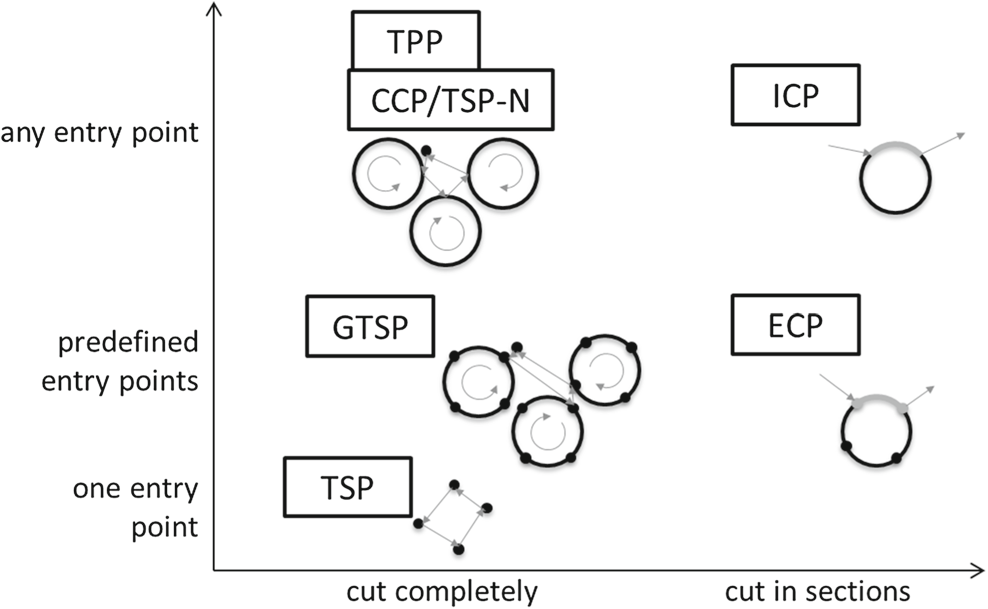
\includegraphics[width=0.9\textwidth]{dewil.png}
  \caption{
    Основные классы задач маршрутизации инструмента
    для машин фигурной листовой резки
  }
  \label{dewil}
\end{figure}

Обычно предполагается также,
что точки врезки в материал,
которые из-за технологических требований резки
(\ref{pierce-constraint})
не совпадают с точками входа в контур,
однозначно определяются выбранными точками входа в контуры (и наооборот)
и находятся от контуров на фиксированном расстоянии.
Отметим, что число сегментов резки
$K$ в кортеже (\ref{tuple})
$ROUTE = \left<
  M_0, M_1, S_1, M_1^*, M_2, S_2, M_2^*, \,\dots, M_K, S_K, M_K^*,
  i_1, i_2, \,\dots, i_K
\right>
$
для первых трех классов задач маршрутизации всегда равно количеству вырезаемых контуров
$N$.

Введем следующее определение.

\begin{opred}
  \label{def:base-segment}
  {\bf Базовым сегментом резки}
  $B^S$
  для сегмента резки
  $S=MM^*$
  будем называть часть траектории сегмента,
  не содержающую траектории входа в контур
  {\it lead-in} и выхода из контура {\it lead-out},
  т.е.
  \begin{equation}
    S=MM^* = M \, lead_{in} \, B^S \, lead_{out} \, M^*
    .
    \label{base-segment}
  \end{equation}
\end{opred}

Будем полагать,
что базовый сегмент,
в отличие от сегмента резки,
не имеет направления,
но тогда если базовый сегмент содержит
один или более замкнутых контуров,
то при определении сегмента резки $S$
нам необходимо для каждого контура задать направление резки
(<<+>> при резке по часовой стрелке,
<<->> против часовой).

Таким образом,
каждый базовый сегмент резки
содержит список
$L(B^S)$
своих замкнутых контуров (может быть пустой).
Пусть
$|L(B^S)|$ --
длина этого списка, тогда кортеж $ROUTE$ (\ref{tuple})
в терминах базового сегмента резки запишется в следующем виде:

\begin{multline}
  ROUTE =  \langle
    M_0, M_1 B^{S_1} M_1^* p_1^1 \,\dots, p_1^{|L(B^{S_1})|},
    M_2 B^{S_2} M_2^* p_2^1 \,\dots, p_2^{|L(B^{S_2})|},
    \\ \dots, \\
    M_K B^{S_K} M_K^* p_K^1 \,\dots, p_K^{|L(B^{S_K})|},
    \\
    i_1, i_2, \,\dots, i_K
  \rangle
  ,
  \label{tuple-base-segments}
\end{multline}
где $p_t^r=\pm 1$
(направление резки в контуре с номером $r$ базового сегмента $B^{S_t}$),
$r=\overline{1, |L(B^{S_t})|}$.

Формула (\ref{tuple-base-segments})
дает наиболее общее формальное описание маршрута резки (траектории интрумента)
машины листовой резки с ЧПУ.

В примере резки двух деталей
на рис.~\ref{cut2-1}
два базовых сегмента выделены пунктирными
желтой и коричневой линиями
(использована мультиконтурная техника резки).

\begin{figure}[H]
  \centering
  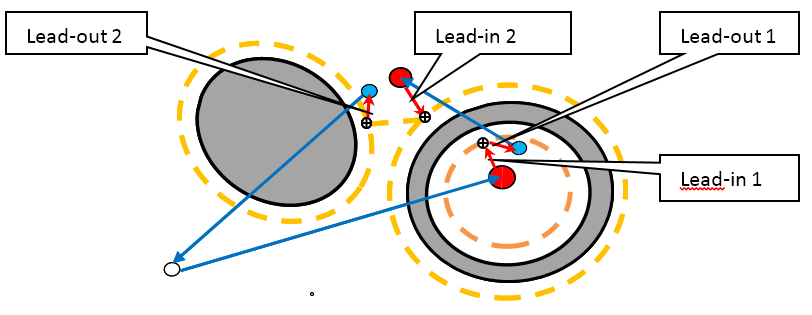
\includegraphics[width=0.9\textwidth]{cut2-1.png}
  \caption{
    Пример схемы резки трех замкнутых контуров
    с использованием двух~сегментов резки
  }
  \label{cut2-1}
\end{figure}

Пример сегмента резки, в котором использована техника совмещенного реза,
и базового сегмента, содержащего четыре контура,
приведен на рис.~\ref{cut4-3}.
Стрелками отмечено направление резки контуров.

\begin{figure}[H]
  \centering
  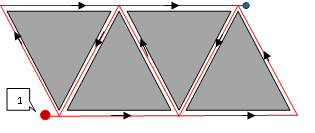
\includegraphics[width=0.7\textwidth]{cut4-3.png}
  \caption{
    Сегмент резки, включающий базовый сегмент
    с использованием техники~резки <<совмещенный рез>>
  }
  \label{cut4-3}
\end{figure}

На основе концепции базового сегмента введем еще
два класса задач маршрутизации инструмента машин
фигурной листовой резки с ЧПУ

\begin{opred}
  \label{def:SCCP}
  {\it SCCP (Segment Continuous Cutting Problem)}
  --
  задача с фиксированным числом $K$
  сементов резки
  (и базовых сегментов резки
  $B^{S_k}, k = \overline{1, K}$).
\end{opred}

{\it Замечание}:
Если все граничные контуры деталей
$C_1, C_2 \,\dots, C_N$
это базовые сегменты $B^{S_k}, k = \overline{1,K}$,
и $N=K$,
тогда $SCCP$ эквивалентна $CCP$.

Предположим, что для исходной задачи маршрутизации
определен конечный набор (ансамбль)
базовых сегментов резки размерности $T$.
Этот ансамбль соответствует ансамблю задач
$\{SCCP_i, i =\overline{1,T}\}$.

\begin{opred}
  {\it GSCCP (Generalized SCCP)} -- есть
  $\{SCCP_i, i =\overline{1,T}\}$.
\end{opred}

Как нетрудно видеть,
введя классы $SCCP$ и $GSCCP$,
мы значительно расширили существующую
классификацию задач маршрутизации инструмента
для машин листовой резки с ЧПУ.
Фактически $SCCP$ и $GSCCP$ являются подклассами $ICP$,
содержащими все задачи с конечным набором базовых сегментов резки,
т. е.
$CCP \subset SCCP \subset GSCCP \subset ICP$.
Таким образом, в классе $ICP$ выбран большой подкласс
задач маршрутизации,
для которых можно разработать эффективные алгоритмы оптимизации.

На рис.~\ref{x-classify}
приведена расширенная классификация этих задач.
Как видно из данного  рисунка,
все классы сгруппированы в три группы,
различающиеся мощностью множеств,
из которых выбираются точки входа в контуры
(точки врезки).

Далее рассмотрим подход,
основанный на  дискретизации трех клаcсов задач маршрутизации
первой группы ({\it CCP, SCCP, GSCCP})
и сведении их к задаче о последовательном обходе мегаполисов,
в которой  используется математическая модель А. Г. Ченцова,
описанная подробно во второй части настоящей монографии
(главы 3 -- 5).

\begin{figure}[H]
  \centering
  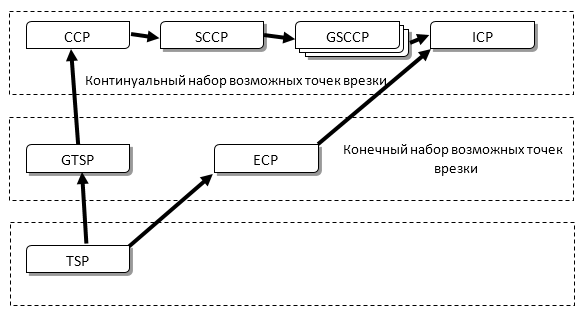
\includegraphics[width=0.9\textwidth]{x-classify.png}
  \caption{
    Расширенная классификация задач
    маршрутизации инструмента машин листовой резки
  }
  \label{x-classify}
\end{figure}

Эта модель может быть интерпретирована
как математическая модель обобщенной задачи коммивояжера ($GTSP$)
с дополнительными ограничениями.
(Следует различать модель $GTSP$
и~задачу маршрутизации $GTSP$ из второй группы,
которая представляеи собой дискретный вариант задачи $CCP$).
В отличие от классического $GTSP$ эта модель
предусматривает учет так называемой внутренней работы
(в данном случае -- процесса резки).
Кроме того, модель мегаполисов с
использованием специальной схемы динамического программирования
учитывает сложные типы целевых функций и сложные ограничения,
в том числе динамические.
Наконец, принимая во внимание ограничения предшествования,
можно получить точные решения для дискретных вариантов $SCCP$
достаточно большой размерности.

В качестве примера рассмотрим задачу $GSCCP$,
которая содержит две
задачи $SCCP$ с разными наборами сегментов,
показанными на рис.~\ref{gsccp-both}
(21 базовый сегмент -- \ref{gsccp-a}
и 18 -- \ref{gsccp-b} соответственно).

Первый набор базовых сегментов,
рис.~\ref{gsccp-a},
задан всеми граничными контурами деталей, т. е.
$C_j = B^{S_j}, j=\overline{1,N}, N=K=21$.
В этом случае мы имеем классическую задачу $CCP$.
На рис.~\ref{gsccp-b} восемь
базовых сегментов заданы внешними граничными контурами <<серых>> деталей.
Три дополнительных базовых сегмента заданы шестью
внешними граничными контурами <<цветных>> деталей
(один базовый сегмент состоит из двух внешних контуров плюс перемычка между ними).
Эти контуры будут вырезаться <<цепной>> резкой попарно в одном базовом сегменте.
Наконец семь базовых сегментов заданы внутренними
граничными контурами всех деталей,
в которых имеются отверстия.
В целом, в этом случае мы имеем набор из восемнадцати
базовых сегментов.
Все они выделены цветом.

\begin{figure}[H]
  \centering
  \subfigure[]{
    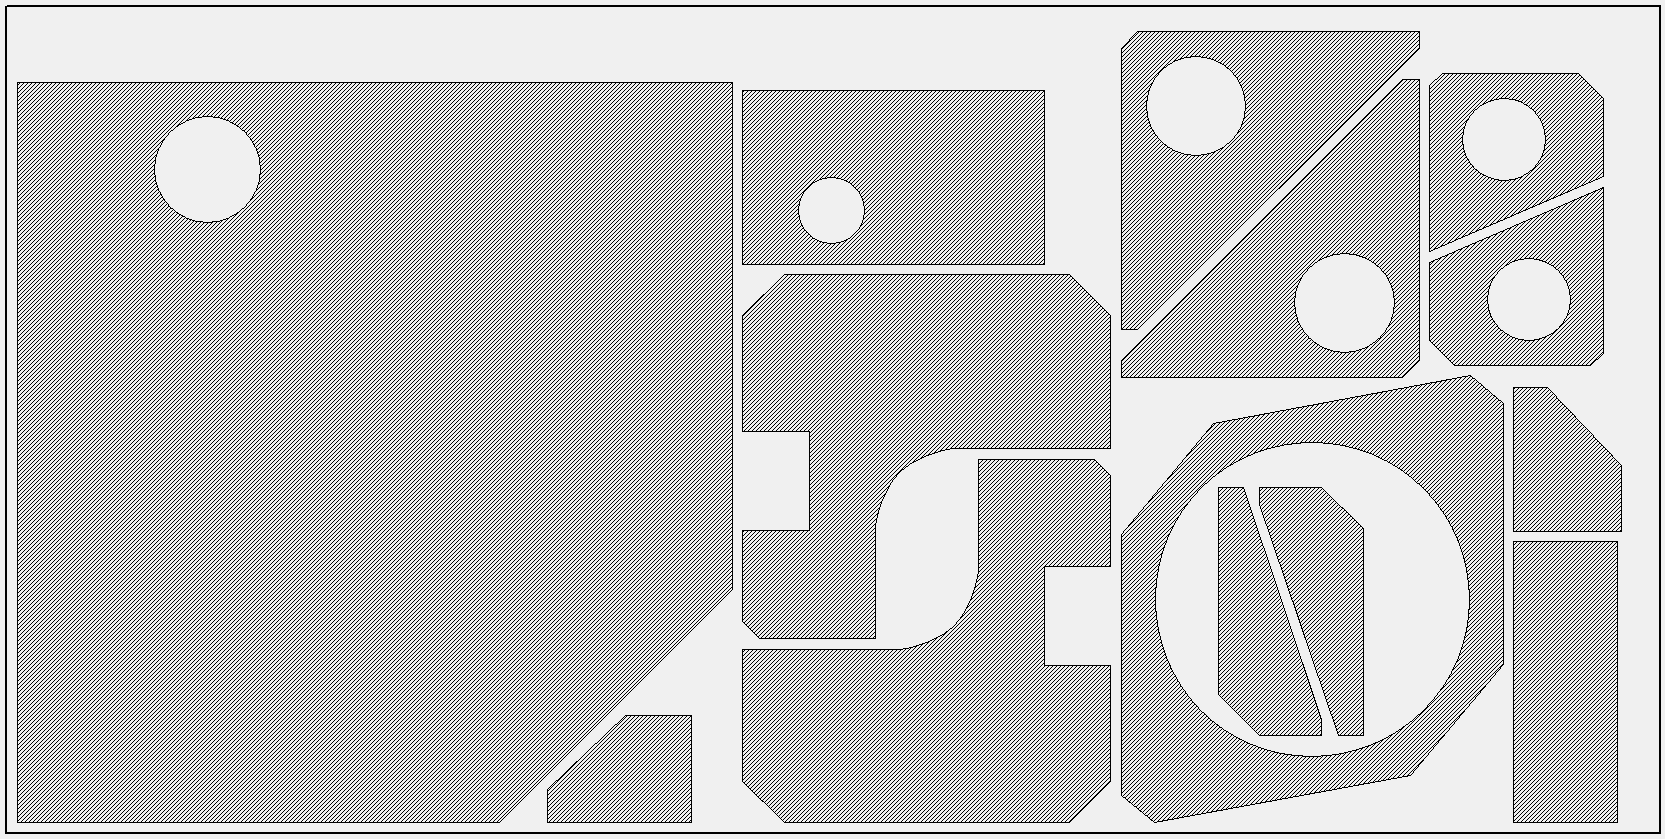
\includegraphics[width=0.9\textwidth]{gsccp-a.png}
    \label{gsccp-a}
  }
  \subfigure[]{
    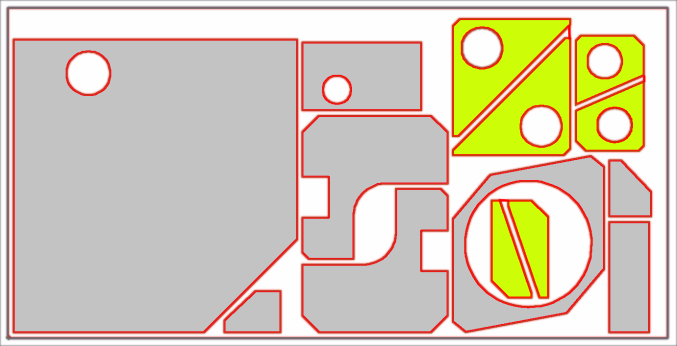
\includegraphics[width=0.9\textwidth]{gsccp-b.png}
    \label{gsccp-b}
  }
  \caption{
    Пример задачи GSCCP с набором из двух комплектов базовых~сегментов: \\
    {\it а} -- 21 базовый сегмент;
    {\it б} -- 18 базовых сегментов
    }
  \label{gsccp-both}
\end{figure}

В качестве целевой функции для данного примера было выбрано
время процесса резки~(\ref{cutting-time}):
$$
  T_{cut} = \frac{L_{on}}{V_{on}} + \frac{L_{off}}{V_{off}} +N_{pt} \cdot t_{pt}
  .
$$

Чтобы свести непрерывные задачи $SCCP$
к дискретной модели,
каждый базовый сегмент делится с определенным шагом по точкам,
которые будут претендентами на точку входа инструмента в контур.
Каждая такая точка входа однозначно определяет точку врезки.
В то же время каждая возможная точка врезки должна
удовлетворять технологическим ограничениям процесса резки
(\ref{pierce-constraint}),
то есть многие точки базовых сегментов будут удалены.
Напомним, что для каждого базового сегмента
такая точка может быть только одна.
На рис.~\ref{discrete21}
показано конечное множество возможных точек врезки
(выделены зеленым цветом)
для первой задачи
(набор из двадцати одного базового сегмента).
Фактически мы свели первую задачу $SCCP$
(в данном конкретном случае эквивалентную $CCP$)
(рис.~\ref{gsccp-a})
к задаче о последовательном обходе мегаполисов (модели $GTSP$).
Обратите внимание,
что в этом случае число возможных маршрутов резки $ROUTE$
становится конечным.
Процесс дискретизации второй задачи SCCP,
рис.~\ref{gsccp-b},
производится аналогичным образом.
Для решения обеих задач применен метод динамического программирования,
использующий специальную схему Беллмана,
которая описана во второй части монографии.

\begin{figure}[H]
  \centering
  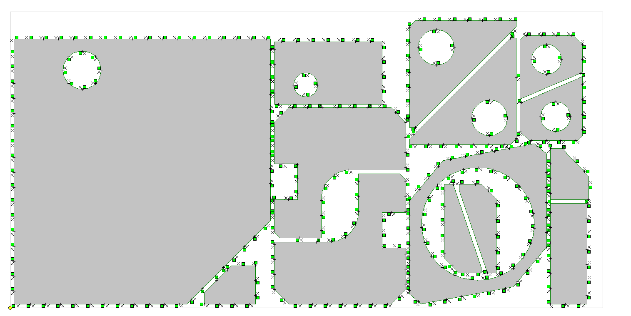
\includegraphics[width=0.9\textwidth]{discrete21.png}
  \caption{
    Дискретизация задачи CCP
    для случая 21 базового сегмента
  }
  \label{discrete21}
\end{figure}

На рис. \ref{gsccp.paths}
показаны оптимальные маршруты резки для двух задач SCCP
с двацать одним и восемнадцатью
базовыми сегментами соответственно.

\begin{figure}[H]
  \centering
  \subfigure[]{
    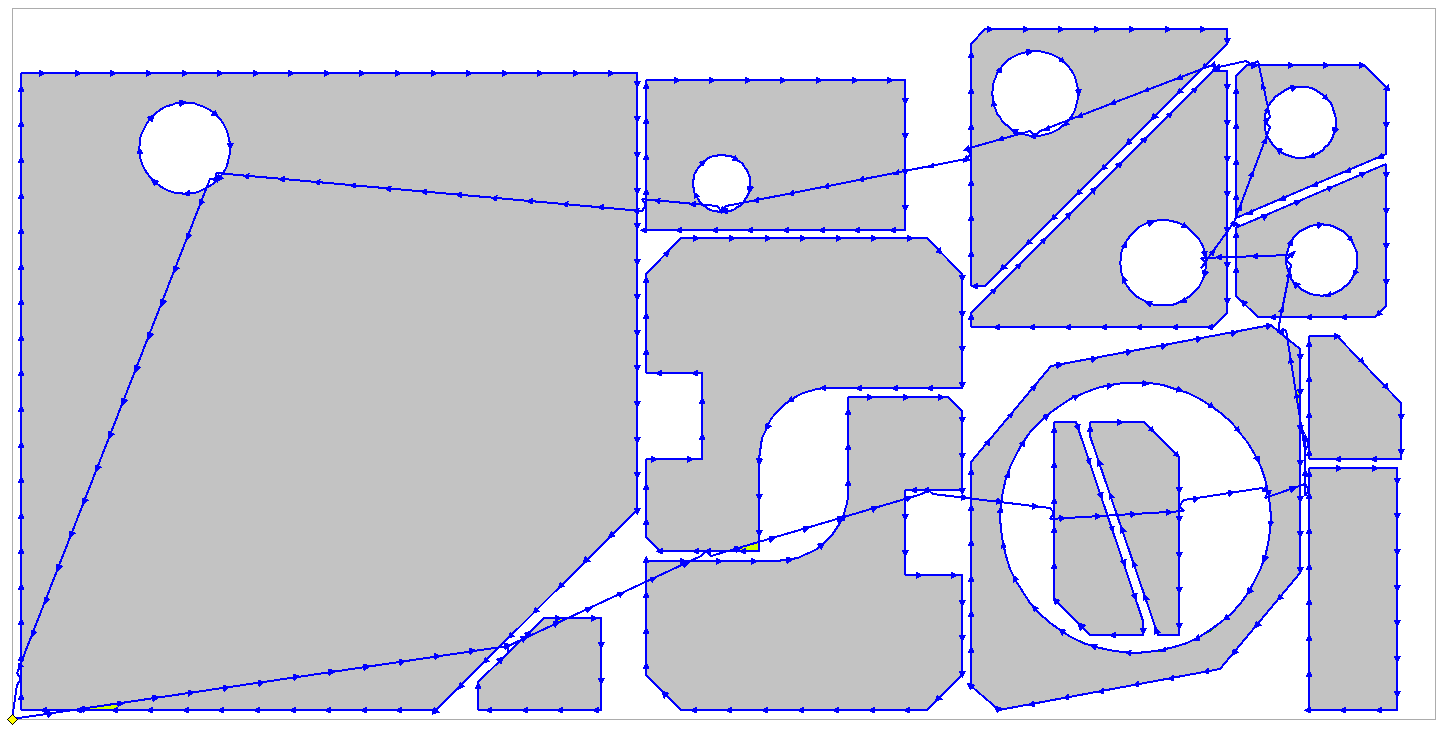
\includegraphics[width=0.9\textwidth]{path21.png}
    \label{path21}
  }
  \subfigure[]{
    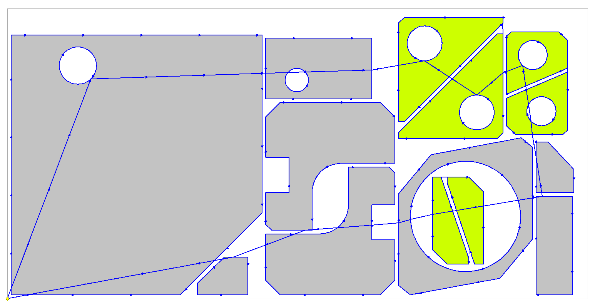
\includegraphics[width=0.9\textwidth]{path18.png}
    \label{path18}
  }
  \caption{
    Схема оптимальной траектории инструмента: \\
    {\it а} -- 21 базовый сегмент;
    {\it б} -- 18 базовых сегментов
  }
  \label{gsccp.paths}
\end{figure}

В первом случае время процесса резки
$T_{cut}$
составляет 2255 с,
во втором -- 2244 с.
Обратите внимание, что в первом случае длина рабочего хода инструмента
$L_{on}$
(20567 мм) меньше, чем во втором -- (20727 мм),
но из-за уменьшения количества точек врезки
для восемнадцати сегментов общее время резки также уменьшилось.
Еще раз отметим, что оба решения являются оптимальными
для выбранных наборов базовых сегментов.
Таким образом, оптимальное значение целевой
функции для выбранной задачи $GSCCP$ составляет 2244 с.

При решении задач были учтены необходимые <<статические>> ограничения:
условия предшествования и ограничения для координат
точек врезки (\ref{pierce-constraint}).
Динамические ограничения в этом модельном примере не рассматривались.

Описанный подход позволяет решать задачи из
наиболее сложного класса задач маршрутизации
траектории инструмента -- $ICP$,
который не ограничивает выбор точки входа
инструмента в контур детали и использование
любой техники резки.
Наиболее важной особенностью подхода
является возможность для одной задачи оптимизации
формировать разные наборы базовых сегментов и
применять разные алгоритмы оптимизации,
используя как дискретные, так и,
в некоторых случаях, непрерывные модели.

